\documentclass{beamer}

\mode<presentation>
{
  \usetheme{Antibes}
  \usecolortheme{beaver}
  % or ...

  \setbeamercovered{transparent}
  % or whatever (possibly just delete it)
}


\usepackage[english]{babel}
\usepackage[utf8]{inputenc}
\usepackage{times}
\usepackage[T1]{fontenc}
\usepackage{graphicx}
\usepackage[compatibility=false]{caption}
\usepackage{subcaption}
\usepackage{physics}
\usepackage{amsmath}
\usepackage{amssymb}

%\usepackage{multimedia}
%\usepackage{movie9}


\newcommand{\expv}[1]{\ensuremath{\mathbb{E}[ #1]}}
\newcommand{\xs}[2]{\ensuremath{\Sigma_{#1}^{(#2)}}}
\newcommand{\intO}{\ensuremath{\int\limits_{4\pi}}}
\newcommand{\intz}{\ensuremath{\int\limits_0^1}}
\newcommand{\intf}{\ensuremath{\int\limits_{-\infty}^\infty}}
\newcommand{\intzf}{\ensuremath{\int\limits_{0}^\infty}}

\title[UQ in RAVEN] % (optional, use only with long paper titles)
{Advanced Methods in \\Stochastic Collocation for Polynomial Chaos\\in RAVEN}

%\subtitle
%{A Term Project}

\author[Talbot] % (optional, use only with lots of authors)
{Paul W. Talbot}%\inst{1}}


\institute[University of New Mexico] % (optional, but mostly needed)
{
  %\inst{1}%
  University of New Mexico%\\
  %\inst{2}
  %Idaho National Laboratory
}

\date[Jan 22 2016] % (optional, should be abbreviation of conference name)
{Dissertation Proposal, January 22nd 2016}


\subject{Uncertainty Quantification}

\pgfdeclareimage[height=0.5cm]{university-logo}{../../graphics/unmlogo}
%\logo{\pgfuseimage{university-logo}}
\logo{\makebox[0.95\paperwidth]{
  
\includegraphics[height=1cm]{../../graphics/INL}\hfill
    
\includegraphics[height=0.5cm]{../../graphics/unmlogo}}

}

\addtobeamertemplate{navigation symbols}{}{
  \usebeamerfont{footline}%
  \usebeamercolor[fg]{footline}%
  \hspace{1em}%
  \insertframenumber/\inserttotalframenumber
}

\begin{document}

\begin{frame}
  \titlepage
\end{frame}

%%%%%%%%%%%%%%%%%%%%%%%%%
%        OUTLINE        %
%%%%%%%%%%%%%%%%%%%%%%%%%

\begin{frame}{Outline}{Discussion Points}\vspace{-20pt}
  \tableofcontents[hideallsubsections]%[pausesections]
  % You might wish to add the option [pausesections]
\end{frame}

%%%%%%%%%%%%%%%%%%%%%%%%%%%%
%        BACKGROUND        % 10 minutes
%%%%%%%%%%%%%%%%%%%%%%%%%%%%
\section{Background}

\subsection{Raven}
\begin{frame}{Background}{RAVEN}\vspace{-20pt}
  \begin{itemize}
    \item Risk Analysis Virtual ENvironment
    \item Verification and Validation
    \item Uncertainty Quantification
    \item Response Surfaces, Risk
    \item Non-Intrusive, Event Trees
  \end{itemize}
\end{frame}
\subsection{Introduction}
% describe uq in general
% introduce terminology
\subsection{Intrusiveness}
% Galerkin/Adjoint methods vs non-intrusive
\subsection{Sampling Strategies}
% Monte Carlo and LHS
% gPC

\begin{frame}{Background}{todo}
  todo
\end{frame}

%%%%%%%%%%%%%%%%%%%%%%%%%%%%
%         METHODS          % 20-30 minutes
%%%%%%%%%%%%%%%%%%%%%%%%%%%%
\section{Methods}
\begin{frame}{Methods}{Outline}\vspace{-20pt}
  \tableofcontents[currentsection]
\end{frame}
\subsection{Physics Models}
\subsubsection{Tensor Polynomials}
\subsubsection{Attenuation}
\subsubsection{Neutron Diffusion}

\subsection{UQ Methods}
\subsubsection{SC for gPC}
\subsubsection{Polynomial Index Sets}
\subsubsection{Sparse Grid Quadrature}
\subsubsection{Adaptive Sparse Grid}

\begin{frame}{Methods}{todo}
  todo
\end{frame}

%%%%%%%%%%%%%%%%%%%%%%%%%%%%
%        PROPOSAL          % 15-20 minutes
%%%%%%%%%%%%%%%%%%%%%%%%%%%%
\section{Proposal}

\subsection{HDMR}
\subsection{AHDMR}
\subsection{Mammoth}
\subsubsection{RattleS$_\text{N}$ake}
\subsubsection{Bison}

\begin{frame}{Proposal}{todo}
  todo
\end{frame}

\end{document}















\section{Sources of Uncertainty}
\begin{frame}{Introduction}{Who is this guy?}\vspace{-30pt}
Current: 
\begin{itemize}
\item  Ph.D Nuclear Engineering student, UNM
\item  Idaho National Laboratory (RAVEN, MOOSE)
\end{itemize}
Past: 
\begin{itemize}
\item M.S. Nuclear Engineering, Oregon State University
\item B.S. Physics, BYU-Idaho (2010)
\end{itemize}
\end{frame}

\begin{frame}{RAVEN}{...and its place in the herd.}\vspace{-20pt}
MOOSE herd
\begin{itemize}
\item \texttt{MARMOT}: Mesoscale materials
\item \texttt{BISON}: Engineering-scale materials
\item \texttt{RattleSNake}: Neutronics
\item \texttt{RELAP-7}: Thermal Hydraulics
\end{itemize}\vspace{10pt}
A different kind of critter...
\begin{itemize}
\item \texttt{RAVEN}: Uncertainty Quantification
\end{itemize}
\end{frame}

\begin{frame}{Uncertainty}{Two Types}\vspace{-30pt}
\begin{itemize}
\item Epistemic - Unmeasured Uncertainty
  \begin{itemize}
  \item Tool Accuracy
  \item Complicated Dependencies (arrow, double pendulum)
  \item Documentation
  \end{itemize}\vspace{20pt}
\item Aleatory - True Randomness
\begin{itemize}
  \item Quantum effects
  \item Particle-Material interactions (gold foil)
  \item Brownian Motion
\end{itemize}
\end{itemize}
\end{frame}

\begin{frame}{Example Stochastic Problem}{Projectile Motion}\vspace{-30pt}
\begin{equation*}
y(t)=y_i + v\sin(\theta)t - \frac{1}{2}gt^2,
\end{equation*}
\begin{equation*}
x(t)=v\cos(\theta)t.
\end{equation*}
%  \begin{figure}[h!]
%    \centering
%      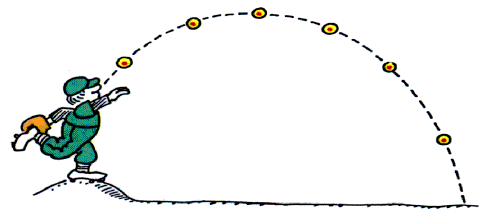
\includegraphics[width=0.5\textwidth]{../graphics/projectile}
%  \end{figure}
%\vspace{-10pt}
Solution: $x_f=\frac{v\cos{\theta}}{g}\left(v\sin\theta+\sqrt{v^2\sin^2\theta + 2gy_i}\right)$
\end{frame}

\begin{frame}{Example Stochastic Problem}{Solved...?}\vspace{-50pt}
\begin{equation*}
x_f=\frac{v\cos{\theta}}{g}\left(v\sin\theta+\sqrt{v^2\sin^2\theta + 2gy_i}\right)
\end{equation*}
\begin{itemize}
\item initial height $y_i = 2$ m
\item initial velocity $v = 35$ m/s
\item initial trajectory $\theta = 35^o$
\item accel. gravity $g = 9.81$ m/s/s
\end{itemize}
Solution: $x_f\approx120$ m
\end{frame}

\begin{frame}{Example Stochastic Problem}{...I'm not so certain anymore.}\vspace{-50pt}
\begin{equation*}
x_f=\frac{v\cos{\theta}}{g}\left(v\sin\theta+\sqrt{v^2\sin^2\theta + 2gy_i}\right)
\end{equation*}
\begin{itemize}
\item initial height $y_i = 1\pm1$ m
\item initial velocity $v = 35.5\pm2.5$ m/s
\item initial trajectory $\theta = 45\pm10^o$
\item accel. gravity $g = 9.7988 \pm0.0349$ m/s/s
\end{itemize}
Solution: $x_f$=?
\end{frame}

\begin{frame}{Uncertainty Quantification}{Methods}\vspace{-20pt}
Some way to quantify uncertainty:
\visible<2->{
\begin{itemize}\vspace{10pt}
\item Min-Max
  \begin{itemize}
  \item Good for monotonic problems
  \end{itemize}\vspace{10pt}}
\visible<3->{
\item Sandwich Formula
  \begin{itemize}
  \item Good for analytic solutions
  \end{itemize}\vspace{10pt}}
\visible<4->{
\item Perturbation
  \begin{itemize}
  \item Valid for small uncertainty
  \end{itemize}
\end{itemize}}
\end{frame}

\section{Analytic Methods}
\begin{frame}{Uncertainty Quantification}\vspace{-20pt}
\[x_f=\frac{v\cos{\theta}}{g}\left(v\sin\theta+\sqrt{v^2\sin^2\theta + 2gy_i}\right)\]
Min-Max
\tiny
\[x_{f,\text{min}}=\frac{(33)(0.5736)}{9.8337}\left((33)(0.8192)+\sqrt{(33)^2(0.8192)^2+2(9.8337)(0)}\right)= 105.46 \text{ m}\]
\[x_{f,\text{max}}=\frac{(55)(0.8192)}{9.7369}\left((55)(0.5736)+\sqrt{(55)^2(0.5736)^2+2(9.8337)(2)}\right)= 142.17 \text{ m}\]
\normalsize
Result: $x_f\approx124\pm18.3$ m \vspace{15pt}\\ \pause
\visible<2->{Flawed Reasoning
\begin{itemize}
\item $\theta$ not monotonic!
\item Does increasing $\theta$ make a longer or shorter range?
\end{itemize}}
\end{frame}

\begin{frame}{Uncertainty Quantification}\vspace{-20pt}
Sandwich Formula (simplified):
\begin{equation*}
\sigma_{x_f} = \sqrt{\left(\pdv{x_f}{y_i}\right)^2\sigma_{y_i}^2 + \left(\pdv{x_f}{v}\right)^2\sigma_{v}^2 + \left(\pdv{x_f}{g}\right)^2\sigma_{g}^2 + \left(\pdv{x_f}{\theta}\right)^2\sigma_{\theta}^2}
\end{equation*}
Works well for simple functions
\begin{itemize}
\item Simple derivatives
\item Analytic solution
\item Assumes mean is reference value
\end{itemize}
\end{frame}

\begin{frame}{Uncertainty Quantification}\vspace{-30pt}
\begin{equation*}
x_f=\frac{v\cos{\theta}}{g}\left(v\sin\theta+\sqrt{v^2\sin^2\theta + 2gy_i}\right)
\end{equation*}%\vspace{10pt}
Sandwich Formula:
\[\sigma_{x_f} = \sqrt{\left(\pdv{x_f}{y_i}\right)^2\sigma_{y_i}^2 + \left(\pdv{x_f}{v}\right)^2\sigma_{v}^2 + \left(\pdv{x_f}{g}\right)^2\sigma_{g}^2 + \left(\pdv{x_f}{\theta}\right)^2\sigma_{\theta}^2}\]% \vspace{20pt}\\
Result: $x_f=120\pm62.44$ m  \vspace{10pt}\\
\end{frame}


\begin{frame}{A More Difficult Problem}{Air Resistance}
%No Air Resistance:
%\begin{equation}
%y_f=v\sin(\theta)t - \frac{1}{2}gt^2,
%\end{equation}
%\begin{equation}
%x_f=v\cos(\theta)t.
%\end{equation}
\vspace{-20pt}With Air Resistance:
\begin{equation*}
y(t)=\frac{v_T}{g}(v\sin\theta+v_T)\left(1-e^{-gt/v_T}\right)-v_Tt,
\end{equation*}
\begin{equation*}
x(t)=\frac{vv_T\cos\theta}{g}\qty(1-e^{-gt/v_T}).
\end{equation*}
\begin{equation*}
v_T=\frac{mg}{D},\hspace{20pt}D=\frac{\rho C A}{2},\hspace{20pt}A=\pi r^2
\end{equation*}
\hspace{30pt}Solve numerically to get $x_f$ (Forward Euler).
\end{frame}

\begin{frame}{A More Difficult Problem}{Aside: Forward Euler}
\vspace{-20pt}Take small $\Delta_t$ time steps
\texttt{while $y^t>0$: $t=t+\Delta_t,$}
\begin{align*}
a_{x}^{(t+\Delta_t)} = \frac{-D}{m}v^{(t)}\ v^{(t)}_{x},
        &\hspace{30pt}a_{y}^{(t+\Delta_t)} = -g-\frac{D}{m}v^{(t)}\ v^{(t)}_{x},\\[15pt]
v_{x}^{(t+\Delta_t)} =v_{x}^{(t)}+ a_{x}^{(t+\Delta_t)}\Delta_t,
        &\hspace{30pt}v_{y}^{(t+\Delta_t)} =v_{y}^{(t)}+ a_{y}^{(t+\Delta_t)}\Delta_t,
        \end{align*}
        \begin{align*}
x^{(t+\Delta_t)} &=x^{(t)}+ v^{(t+\Delta_t)}_{x}\Delta_t + \frac{1}{2}a^{(t+\Delta_t)}_{x} \Delta_t^2,\\
y^{(t+\Delta_t)} &=y^{(t)}+ v^{(t+\Delta_t)}_{y}\Delta_t + \frac{1}{2}a^{(t+\Delta_t)}_{y} \Delta_t^2.
\end{align*}
\hspace{50pt}(video)
\end{frame}

\begin{frame}[label=unc_sum]{A More Difficult Problem}{Uncertainty Summary}\vspace{-30pt}
\begin{align*}
y_i=1&\pm1\text{ m},\\
v=35.5&\pm2.5\text{ m/s},\\
\theta=45&\pm10^o,\\
g=9.7988&\pm0.0349\text{ m/s/s},\\
m=0.145&\pm0.0725\text{ kg},\\
r=0.0336&\pm0.00336\text{ m},\\
C=0.5&\pm0.5,\\
\rho_\text{air}=1.2&\pm0.1\text{ kg/m$^3$}.
\end{align*}
\begin{center}\hyperlink{sens_use}{\beamergotobutton{UQ Uses}}\end{center}\vspace{-20pt}
\begin{center}\hyperlink{sens_res}{\beamergotobutton{Sensitivity Study}}\end{center}
\end{frame}

\begin{frame}{A More Difficult Problem}{Equation Summary}
\begin{equation*}
y(t)=\frac{v_T}{g}(v\sin\theta+v_T)\left(1-e^{-gt/v_T}\right)-v_Tt,
\end{equation*}\vspace{15pt}
\begin{equation*}
x(t)=\frac{vv_T\cos\theta}{g}\qty(1-e^{-gt/v_T}).
\end{equation*}\vspace{15pt}
\begin{equation*}
v_T=\frac{mg}{D},\hspace{20pt}D=\frac{\rho C A}{2},\hspace{20pt}A=\pi r^2
\end{equation*}
\end{frame}

\section{Numerical Methods}
\begin{frame}{Uncertainty Quantification}{Complicated Problems}\vspace{-20pt}
How do we quantify uncertainty for problems without simple analytic solutions?\vspace{15pt}
\begin{itemize}
\item Monte Carlo sampling
\item Stochastic Collocation
%\item High Density Model Reduction (low-order)
\end{itemize}
\end{frame}

\begin{frame}{Uncertainty Quantification}{Monte Carlo}\vspace{-30pt}
\begin{itemize}
\item Let $u(Y)$ be any system, like $x_f(y_i,v,\theta,g,m,r,C,\rho$)
\item Randomly sample input parameters, record outputs
\item Repeat $M$ times
\item Calculate moments (mean, variance, skew, kurtosis)
\end{itemize}
\centerline{Mean: $\bar u\approx\frac{1}{M}\sum u\left(Y^{(m)}\right)$}
(video)
\end{frame}

%\section{Stochastic Collocation}
\begin{frame}{Uncertainty Quantification}{Stochastic Collocation}\vspace{-30pt}
\begin{itemize}
\item Let $u(Y)$ be any system, like $x_f(y_i,v,\theta,g,m,r,C,\rho)$
\item Represent original model with polynomials
\item Calculate moments (mean, variance, skew, kurtosis)
\end{itemize}
\begin{equation*}
u(Y)\approx S[u(Y)]\equiv\sum_{k\in\Lambda}c_k\Phi_k(Y),
\end{equation*}
\begin{equation*}
\Phi_k(Y) = \phi_{k_1}(Y_1)\cdot\phi_{k_2}(Y_2)\cdot\ldots\cdot\phi_{k_N}(Y_N)
\end{equation*}
\end{frame}

\begin{frame}{Uncertainty Quantification}{Stochastic Collocation}\vspace{-20pt}
Our case:
\begin{align*}
x_f(y_i,v,\theta,g,m,r,C,\rho)&\approx S[x_f(y_i,v,\theta,g,m,r,C,\rho)],\\
  &\approx\sum_{k\in\Lambda}c_k\Phi_k(y_i,v,\theta,g,m,r,C,\rho),
\end{align*}
\begin{equation*}
\Phi_k(y_i,v,\theta,g,m,r,C,\rho) = \phi_{y_i}(y_i)\cdot\phi_{v}(v)\cdot\ldots\cdot\phi_{\rho}(\rho).\vspace{10pt}
\end{equation*}
\begin{equation*}
c_k = \frac{\int\int\int\int\int\int\int\int x_f\Phi\ d(y_i,v,\theta,g,m,r,C,\rho)}{\int\int\int\int\int\int\int\int \Phi^2\ d(y_i,v,\theta,g,m,r,C,\rho)}.
\end{equation*}
%For example: $k=(1,1,2,2,3,3,4,4)$ and \\$\phi$ as monomials ($1,x,x^2,x^3,x^4,\ldots$),
%\begin{equation*}
%\Phi_k(y_i,v,\theta,g,m,r,C,\rho) = y_i\cdot v\cdot \theta^2\cdot g^2\cdot m^3\cdot r^3\cdot C^4\cdot \rho^4.
%\end{equation*}
\end{frame}

\begin{frame}{Uncertainty Quantification}{Combining polynomials?}
For example, let $\phi$ be monomials $(1,x,x^2,x^3,x^4,...)$.
\begin{equation*}\small
\Lambda = \left\{
\begin{array}{c}
(0,0,0,0,0,0,0,0), \\
(1,0,0,0,0,0,0,0), \\
(0,1,0,0,0,0,0,0), \\
\ldots \\
(1,2,3,4,5,6,7,8), \\
\ldots \\
\end{array}\right\}
\end{equation*}\normalsize
\begin{table}
\centering
\begin{tabular}{c c}
$k$ & polynomial $\Phi$ \\ \hline
(0,0,0,0,0,0,0,0) &  $y_i^0 \cdot v^0 \cdot \theta^0 \cdot g^0 \cdot m^0 \cdot r^0 \cdot C^0 \cdot \rho^0 = 1$ \\
(1,2,3,4,5,6,7,8) &  $y_i^1 \cdot v^2 \cdot \theta^3 \cdot g^4 \cdot m^5 \cdot r^6 \cdot C^7 \cdot \rho^8$ \\
(1,1,1,1,1,1,1,1) & $ y_i \cdot v \cdot \theta \cdot g \cdot m \cdot r \cdot C \cdot \rho$ \\
\end{tabular}
\end{table}
\end{frame}



\begin{frame}{Uncertainty Quantification}{Stochastic Collocation}\vspace{-20pt}
Comparison
\begin{table}
\centering
\begin{tabular}{c|c}\small
Monte Carlo & Stochastic Collocation \\\hline
Dimension-independent & Calculations grow with dimension* \\
Slow converging & Very fast convergence* \\
 & Can replace original model
\end{tabular}
\end{table}
\end{frame}


%\begin{frame}{Uncertainty Quantification}{Results: Expected Value, Values}
%  \begin{figure}[h!]
%    \centering
%      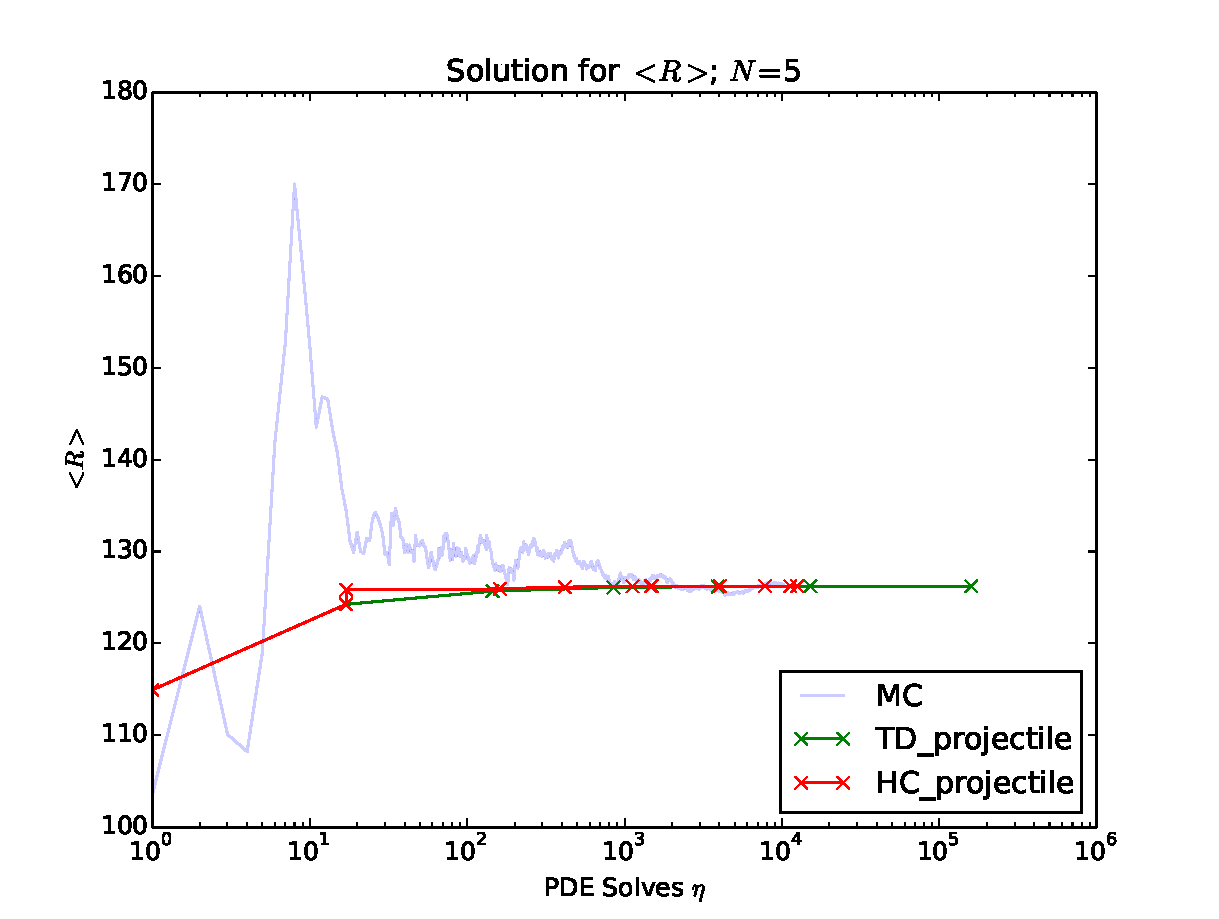
\includegraphics[width=0.7\textwidth]{../graphics/projectile_solns}
%      \caption{$\expv{x_f}$}
%    \begin{subfigure}[b]{0.49 \textwidth}
%      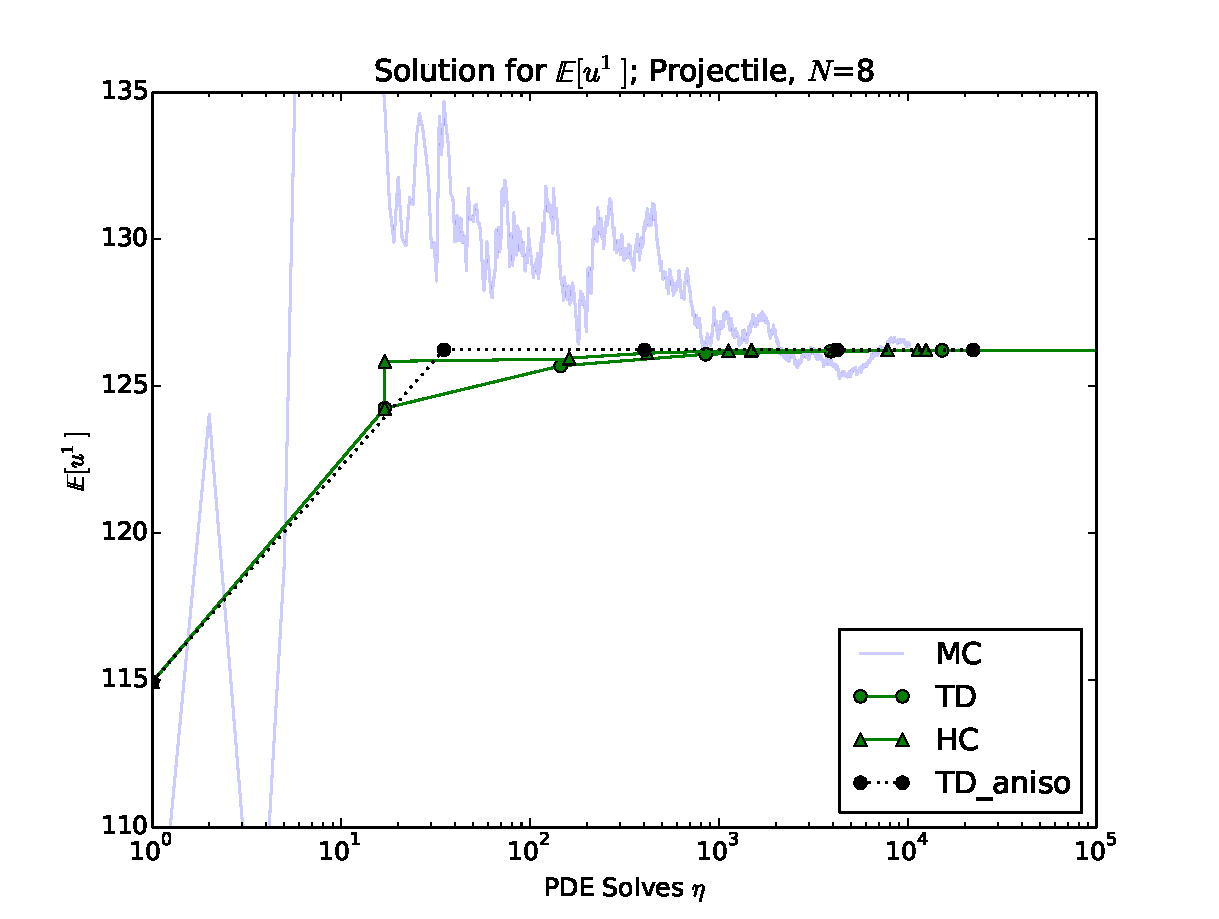
\includegraphics[width=\textwidth]{../graphics/projectile_solns_aniso}
%      \caption{$<R>$ Values}
%      \label{err_5}
%    \end{subfigure}
%    \begin{subfigure}[b]{0.49 \textwidth}
%      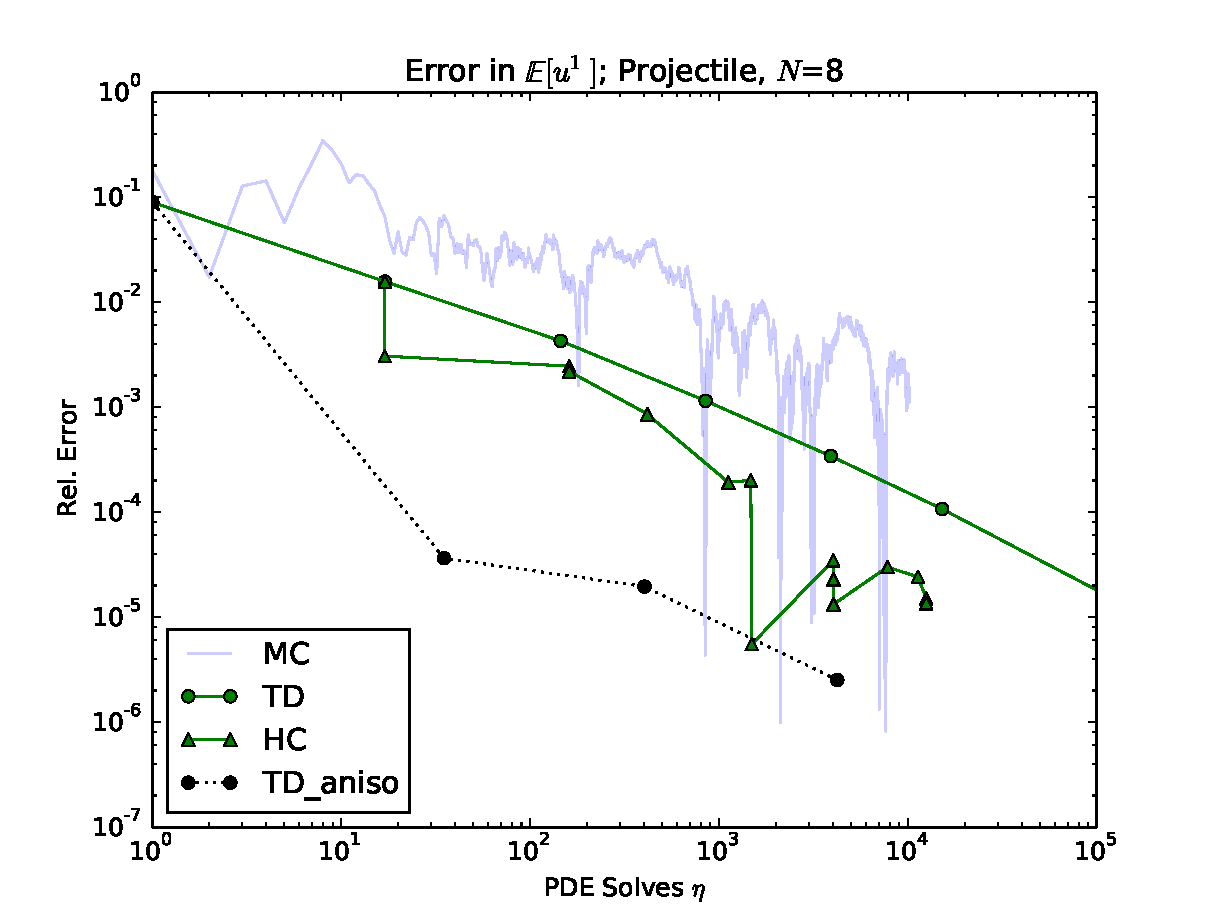
\includegraphics[width=\textwidth]{../graphics/projectile_errs_aniso}
%      \caption{Error in $<R>$}
%      \label{err_14}
%    \end{subfigure}
%  \end{figure}
%\end{frame}

%\begin{frame}{Uncertainty Quantification}{Results: Expected Value, Errors}
%  \begin{figure}[h!]
%    \centering
%      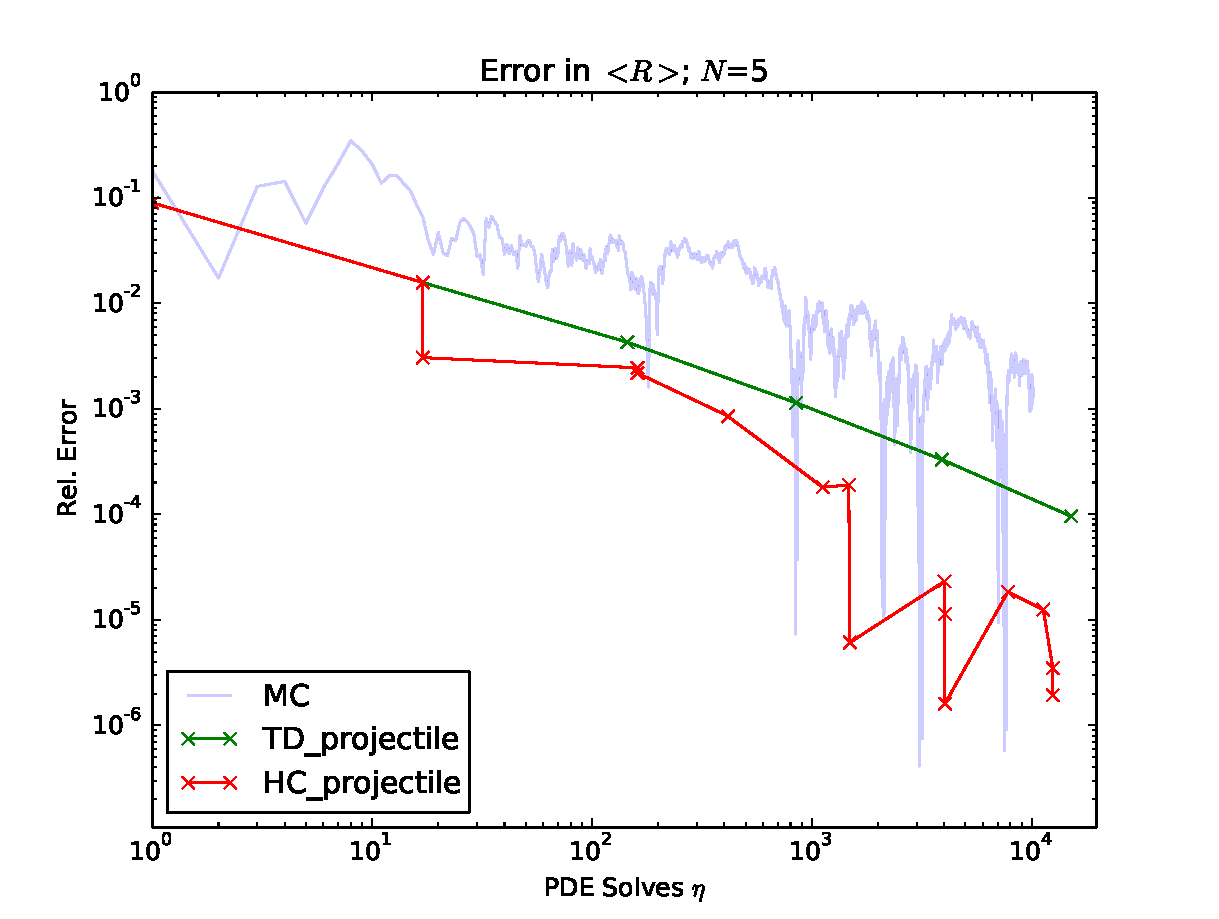
\includegraphics[width=0.7\textwidth]{../graphics/projectile_errs}
%      \caption{Error in $\expv{x_f}$}
%  \end{figure}
%\end{frame}

%\begin{frame}{Uncertainty Quantification}{Results: Second Moment, Values}
%  \begin{figure}[h!]
%    \centering
%      \includegraphics[width=0.7\textwidth]{../graphics/projectile_solns_variance}
%      \caption{$\expv{x_f^2}$}
%  \end{figure}
%\end{frame}
%
%\begin{frame}{Uncertainty Quantification}{Results: Second Moment, Errors}
%  \begin{figure}[h!]
%    \centering
%      \includegraphics[width=0.7\textwidth]{../graphics/projectile_errs_variance}
%      \caption{Error in $\expv{x_f^2}$}
%  \end{figure}
%  \begin{figure}[h!]
%    \centering
%    \begin{subfigure}[b]{0.49 \textwidth}
%      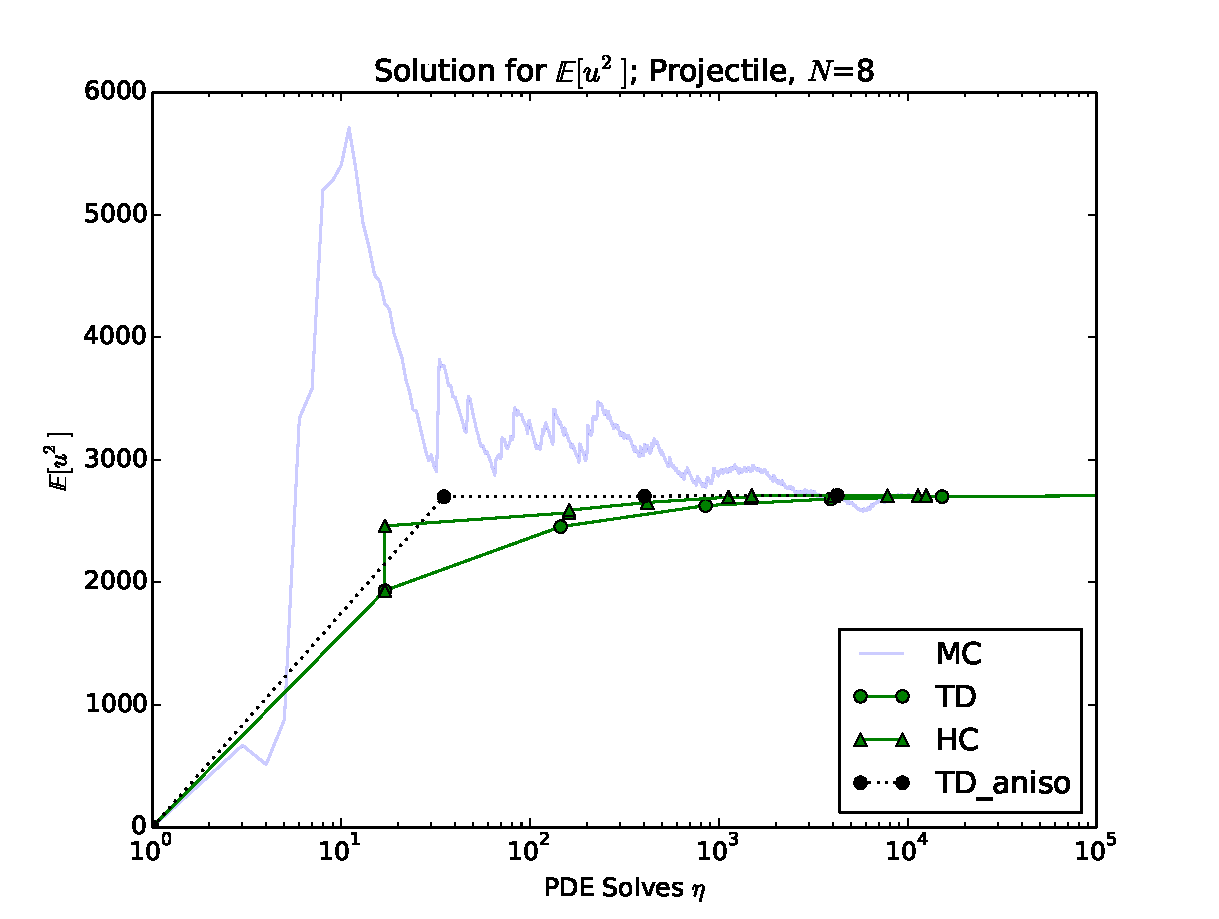
\includegraphics[width=\textwidth]{../graphics/projectile_solns_aniso_variance}
%      \caption{$<R>$ Values}
%      \label{err_5}
%    \end{subfigure}
%    \begin{subfigure}[b]{0.49 \textwidth}
%      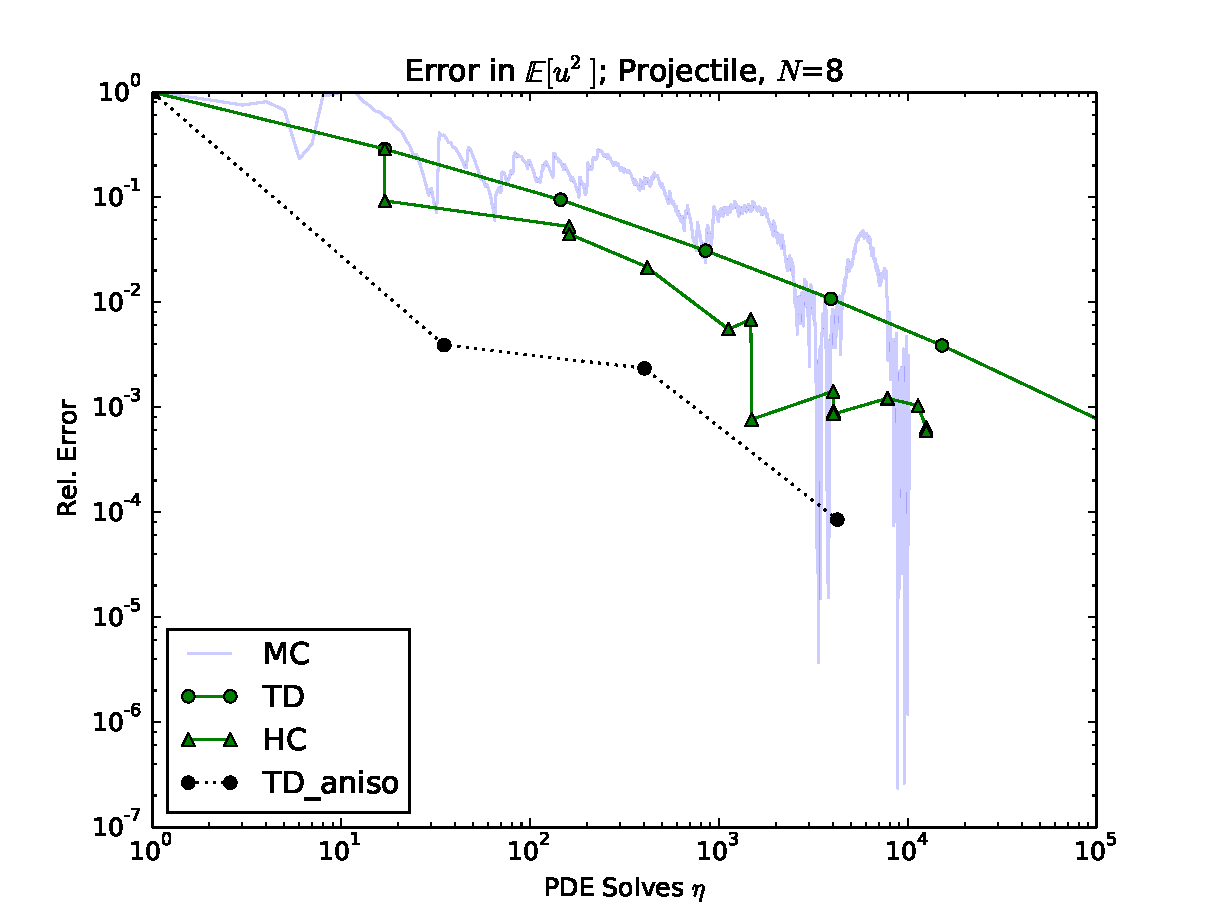
\includegraphics[width=\textwidth]{../graphics/projectile_errs_aniso_variance}
%      \caption{Error in $<R>$}
%      \label{err_14}
%    \end{subfigure}
%  \end{figure}
%\end{frame}

\section{Extra: Sensitivity Analysis}
\begin{frame}[label=sens_use]{Sensitivity Analysis}{So...what?}\vspace{-20pt}
Uses for uncertainty quantification:\vspace{5pt}
\begin{itemize}
\item Understand range of possible solutions
\item Worse-case scenarios
\item Sensitivity Analysis
  \begin{itemize}
  \item Who is contributing the most to our spread?
  \item Which measurements should I focus on improving?
  \item Which design specification should I tighten down on?
  \end{itemize}
\end{itemize}\vspace{-15pt}
\begin{center}\hyperlink{unc_sum}{\beamergotobutton{Inputs}}\end{center}
\end{frame}

\begin{frame}{Sensitivity Analysis}{Polynomial Expansion Revisited}\vspace{-30pt}
Recall: $u(Y)\approx S[u(Y)]=\sum_{k\in\Lambda}c_k\Phi_k(Y),$ 

so for $x_f(y_i,v,\theta,g,m,r,C,\rho)$:
\begin{align*}
&x_f \approx S[x_f]= c_{(0,0,0,0,0,0,0,0)} \\
 &+c_{(1,0,0,0,0,0,0,0)}y_i + c_{(0,1,0,0,0,0,0,0)}v + c_{(0,0,1,0,0,0,0,0)}\theta+\ldots\\
 &+c_{(2,0,0,0,0,0,0,0)}y_i^2 + c_{(1,1,0,0,0,0,0,0)}y_i\cdot v + c_{(1,0,1,0,0,0,0,0)}y_i\cdot \theta +\ldots\\
 &+c_{(3,0,0,0,0,0,0,0)}y_i^3 + c_{(1,1,1,0,0,0,0,0)}y_i\cdot v\cdot\theta +\ldots\\
 &\ldots
\end{align*}
\end{frame}

\begin{frame}{Sensitivity Analysis}{Polynomial Expansion Revisited}\vspace{-30pt}
Rearrange:
\begin{align*}
&x_f \approx S[x_f]=c_{(0,0,0,0,0,0,0,0)} \\
 &+c_{(1,0,0,0,0,0,0,0)}y_i + c_{(2,0,0,0,0,0,0,0)}y_i^2 + c_{(3,0,0,0,0,0,0,0)}y_i^3+\ldots\\
 &+c_{(0,1,0,0,0,0,0,0)}v + c_{(0,2,0,0,0,0,0,0)}v^2 + c_{(0,3,0,0,0,0,0,0)}v^3+\ldots\\
 &\ldots\\
 &+c_{(1,1,0,0,0,0,0,0)}y_i\cdot v + c_{(1,2,0,0,0,0,0,0)}y_i\cdot v^2+\ldots\\
 &\ldots
\end{align*}
\end{frame}

